\documentclass[]{beamer}

\usepackage[T1]{fontenc}
\usepackage[english]{babel}
%\usepackage[utf8]{inputenc}
\usepackage[babel]{csquotes}
\usepackage{graphicx}
\usepackage{lmodern}
\usepackage{textcomp}
\usepackage{booktabs}
\usepackage{tipa}
\usepackage{gb4e}
\noautomath
\usepackage{subfigure}
\usepackage{verbatim}
\usepackage{listings}
\usepackage{hyperref}
\lstset{
  basicstyle=\ttfamily,
  columns=fullflexible,
  showstringspaces=false,
  commentstyle=\color{gray}\upshape
}

\setbeamertemplate{section in toc}[sections numbered]

\setbeamercovered{transparent}
\setbeamertemplate{footline}[frame number]

\usepackage[backend=biber, 
					style=authoryear-comp, %ebd. %keine ebd.: comp, kompakt
						dashed=false,
						sorting=nyt,	%Name, Year, Title
						maxbibnames=13,
						minbibnames=13, % in der Bibliography Anzahl der Namen in Listen
						maxcitenames=2,
						mincitenames=1, % in der Zitation Anzahl der Namen
						isbn=false,
						url=true,
						doi=false,
						eprint=false,
						block=space % horzontaler Platz zw. Feldern
						]{biblatex}



\addbibresource{literature.bib}
\bibliography{literature}
\renewcommand{\bibfont}{\tiny}

%\titlegraphic{}
\title[]{COST Action Distant Reading for European Literary History}
\subtitle[]{European Literary Text Collection (ELTeC) \\ 

\includegraphics[scale=0.35]{pics/distantreadinglogo-high-300x138.png}
}
\date[]{\small \textcolor[rgb]{0.4,0.4,0.4}{TS Budapest Track 1,  Corpus design and text contribution for ELTeC}}
\author[]{\textcolor[rgb]{0,0,0}{ Christof Sch\"och, Carolin Odebrecht, Lou Burnard, Borja Navarro-Colorado et al.}}
%\institute[]{\textcolor[rgb]{0,0,0}{}}

\begin{document}

%\setcounter{framenumber}{-1}
\frame{
  \titlepage
}

\frame{
\frametitle{TS -- Organisation, schedule and data}

\begin{itemize}
\item \textcolor[rgb]{0,0,1}{\href{https://github.com/distantreading/WG1/wiki/TS-Budapest}{Schedule}}
	\item \textcolor[rgb]{0,0,1}{\href{https://github.com/distantreading/WG1/tree/master/Training/2019-09-budapest}{Slides}}
	\item \textcolor[rgb]{0,0,1}{\href{https://github.com/distantreading/WG1/tree/master/Training/2019-09-budapest}{Training data}}
	\item \textcolor[rgb]{0,0,1}{\href{https://github.com/COST-ELTeC}{Corpus data}}
\end{itemize}

}

\frame{
\frametitle{TS -- Track 1}

\begin{itemize}
\item Introduction to \textsc{ELTeC}
\item Metadata in the \textsc{teiHeader}
\item Optical character recognition
	\item Hands-on experience in creating \textsc{ELTeC} \textsc{TEI}-XML versions of source texts 
	\item Start from scanned page images or from a pre-existing HTML version
	\item TS output: contribute new \textsc{TEI} encoded texts to the \textsc{ELTeC} GitHub repository
\end{itemize} 
}

\begin{frame}
	\frametitle{Outline}
	\tableofcontents
\end{frame}

\section{COST Action \textsc{Distant Reading} and Working Group \textsc{Scholarly Resources}}

\frame{
\frametitle{COST\footnote{European Cooperation in Science and Technology = COST\footnote{\url{www.cost.eu}}
} Action Distant Reading}

\begin{itemize}
	\item Christof Sch\"och, University of Trier
	\item CA16204 will
	\begin{itemize}
		\item \glqq{}create a vibrant and diverse network of researchers jointly developing the resources and methods necessary to change the way European literary history is written\grqq{}
		\item \glqq{}contribute to the development and distribution of methods, competencies, data, best practices, standards and tools relevant to Distant Reading research\grqq{}\footnote{\url{www.distant-reading.net}}
		\item started autumn 2017
	\end{itemize}
	\item Working groups
	\begin{itemize}
		\item WG 1: Scholarly Resources
		\item WG 2: Methods and Tools
		\item WG 3: Literary Theory and History
		\item WG 4: Dissemination
	\end{itemize}
\end{itemize}
}

\frame{
\frametitle{Working Group 1: \textsc{Scholarly Resources}}
\begin{itemize}
	\item Creating an open source multi-lingual benchmark corpus for European literature of the 19th century (novels):
	European Literary Text Collection (\textsc{ELTeC})\footnote{\url{https://www.distant-reading.net/wg-1/}}
	\item 34 Members from 22 countries
	\item Main tasks are
	\begin{itemize}
		\item defining corpus design
		\item developing basic encoding schemas
		\item developing workflows
	\end{itemize}
\end{itemize}
}

\frame{
\frametitle{Working Group 1: \textsc{Scholarly Resources}}

Context of the WG:
\begin{itemize}
	\item closely related to WG2 \textsc{Tools and methods} and WG3 \textsc{Theory}, cf. parallel tracks of the TS
	\item aims to support many different perspectives on distant reading
	\item many members with different scientific background and experience in data creation
	\item enabling distant collaborative work on creating \textsc{ELTeC} 
\end{itemize}
}

\section{\textsc{ELTeC} Corpus Design}
\begin{frame}
	\frametitle{Outline}
	\tableofcontents[currentsection]
\end{frame}

\frame{
\frametitle{Corpus design}

Corpus design defines two things \parencites[cf.][]{LudelingRitzStedeEtAl2016,Hunston2008}:
	\begin{itemize}
		\item candidates $\rightarrow$ sampling
		\begin{itemize}
			\item Which text(s) can be included in the corpus? Which can't?
		\end{itemize}
		\item proportion $\rightarrow$ balancing
		\begin{itemize}
			\item How many texts with which characteristics should the corpus contain? 
		\end{itemize}
	\end{itemize}
}

\frame{
\frametitle{Corpus design -- approach of WG1}

\begin{itemize}
\item Sampling and balancing criteria\footnote{\tiny\url{https://github.com/distantreading/WG1/blob/master/sampling_proposal.xml}} will
\begin{itemize}
	\item not define what a novel is
	\item follow a non-normative but metadata-based approach (not canon-based)\footnote{\tiny Each canon is
                    a result of rating texts from different perspectives: intellectual, economical, or/and reader rating \parencites[a.o.][]{Winko1996,Herrmann2011}.}
	\item aim to represent the variety of a population\footnote{\tiny Cf. for discussion of representativeness \textcite{Biber1993} and canonicity and corpus design \textcites{AlgeeHewittMcGurl2018,BodeKatherine2018AWoF}.}
	\item allow for a comparability of texts and individual sub-collections according to different metadata set(s)
\end{itemize}
\end{itemize}
}

\frame{
\frametitle{Sampling criteria}

\begin{itemize}
	\item \textbf{language}: European languages, no translations
	\item \textbf{prose}: narrative fictional prose
	\item \textbf{period}: 1840--1920
	\item \textbf{length}: min. 10.000 words
		\item \textbf{publication}: prefer books over novels published in serial publications
	\item \textbf{access}: only freely available digitizations
\end{itemize}

}
\frame{
\frametitle{Balancing criteria}

100 texts per language (language collection)
	\begin{itemize}
		\item \textbf{period}: distribution over time
		\begin{itemize}
			\item group T1: 1840-1859
			\item group T2: 1860-1879
			\item group T3: 1880-1899
			\item group T4: 1900-1920
		\end{itemize}
		\item \textbf{gender}: min. 10\% and max. 50\% written by female authors
		\item \textbf{authorship}: 9 - 11 authors with exactly three novels (otherwise, only one text for each author)
		\item \textbf{length}: min. 20\% are short novels (10-50k word tokens), min. 20\% are long novels (>100k word tokens).
		\item \textbf{reprint}: min. 30\% are highly canonized novels, min. 30\% should be non-canonized novels (rarely or never reprinted), based reprint counts within the period 1970-2009 ("unmarked", information not yet available)
	\end{itemize}
}

\frame{
\frametitle{(ideal) Composition}

\begin{figure}%
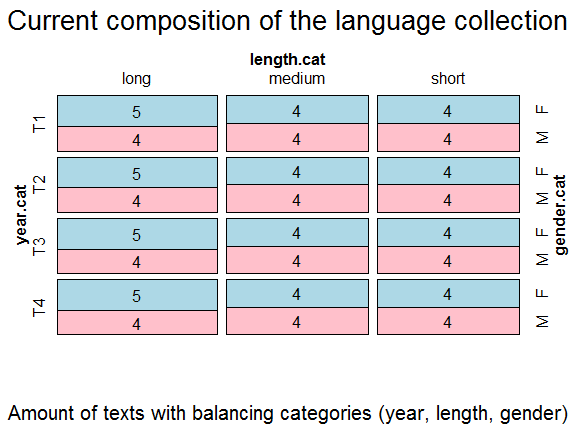
\includegraphics[scale=0.5]{pics/Rplot-balanced.png}%
\end{figure}

ELTeC summary \url{https://distantreading.github.io/ELTeC/}

}

\section{WG Workflow}
\begin{frame}
	\frametitle{Outline}
	\tableofcontents[currentsection]
\end{frame}

\frame{
\frametitle{WG workflow}
\begin{itemize}
	\item WG1 on GitHub{\footnote{\url{https://github.com/distantreading/WG1}}}
	\begin{itemize}
		\item organization and documentation
	\end{itemize}
	\item \textsc{ELTeC} on GitHub\footnote{\url{https://github.com/COST-ELTeC}}
	\begin{itemize}
		\item data and scripts
	\end{itemize}
	\item Archiving on Zenodo\footnote{\url{https://zenodo.org/communities/eltec/}}
\end{itemize}
}

\frame[allowframebreaks]{
\frametitle{References}
\printbibliography
}

\end{document}
